\documentclass[10pt]{article}

\def\Type{LessonDJ}
\def\TypeNum{Workshop Week 5} %Lesson #
\def\TypeTitle{Derivative Shortcuts } %Lesson Title
\def\Semester{Fall 2021} %Not Used 
\def\Course{MATH 1190}%Course number and name
\def\Targets{  \target{D2} }

\usepackage{preambleDJ} 

%%%%%%%%%%%% BEGIN DOCUMENT %%%%%%%%%%%%%%%
%%%%%%%%%%%% BEGIN DOCUMENT %%%%%%%%%%%%%%%
%%%%%%%%%%%% BEGIN DOCUMENT %%%%%%%%%%%%%%%
%%%%%%%%%%%% BEGIN DOCUMENT %%%%%%%%%%%%%%%
%%%%%%%%%%%% BEGIN DOCUMENT %%%%%%%%%%%%%%%

\begin{document}
\pagestyle{otherpages}
\thispagestyle{firstpage}

\vs{.6}
\section{Derivative Rules}
{
\paragraph*{Prompt:} Fill in the following derivatives and derivative rules. You may use the space at the bottom of this sheet of paper for scratch work, but please only write your final answers in the blanks. {\bf You may want to carry this sheet with you for your reference as you rotate from board to board today, so please make sure your answers are legible and correct!}\\[0.1in]

\begin{tabular}{l c r l c r}
            %
            $\displaystyle\frac{d}{dx}\left[ f(x)g(x) \right]$ & $=$ & \rule[-8pt]{2in}{0.4pt} &
            %
            $\displaystyle\frac{d}{dx}\left[ \dfrac{hi(x)}{lo(x)} \right]$ & $=$ & \rule[-8pt]{2in}{0.4pt}\\[0.3in]
            %%%%%
            $\displaystyle\frac{d}{dx}\left[ x^n \right]$ & $=$ & \rule[-8pt]{2in}{0.4pt} & 
            %
            $\displaystyle\frac{d}{dx}\left[ e^x \right]$ & $=$ & \rule[-8pt]{2in}{0.4pt}\\[0.3in]
            %%%%%
            $\displaystyle\frac{d}{dx}\left[ f(g(x)) \right]$ & $=$ & \rule[-8pt]{2in}{0.4pt} & 
            %
            $\displaystyle\frac{d}{dx}\left[ e^{10} \right]$ & $=$ & \rule[-8pt]{2in}{0.4pt}\\[0.3in]
            %%%%%
            $\displaystyle\frac{d}{dx}\left[ \frac{1}{\sqrt[3]{x^2}} \right]$ & $=$ & \rule[-8pt]{2in}{0.4pt} & 
            %
            $\displaystyle\frac{d}{dx}\left[ \frac{1}{x^2} \right]$ & $=$ & \rule[-8pt]{2in}{0.4pt}\\[0.3in]
            %%%%%
        \end{tabular}

%%%%%%%%%
\newpage%
%%%%%%%%%

%%%%%%%%%%%%%%%%%%%%%%%%%%%%%%%%%%%%%%%%%%%%%%
%%% PUT BOARDWORK PROBLEMS AFTER THIS NOTE! %%
%%%%%%%%%%%%%%%%%%%%%%%%%%%%%%%%%%%%%%%%%%%%%%

\section{More Practice}
{\large

  \begin{enumerate}
  \mpageT{.5}{.5}[\hs{.2}]{
    \item $\dfrac{d}{dt}[ t^2 + 2t]$
    \item $\dfrac{d}{dt}\left[\dfrac{2\sqrt{t}-t}{t^2+2t}\right]$
    \item $\dfrac{d}{dt}\left[(t^2+2t)(2\sqrt{t}-t)\right]$
      \item $\ds \dfrac{d}{dt}\left[\frac{t}{g(2t)}\right]_{t=2}$  where $g(2)=-1$, \\\\$g(4)=5$, $g^{\prime}(2)= -7$, $g^{\prime}(4)= 9$ 
}{
    \item $\ds \dfrac{d}{dx}\left[e^{5x^2+7}\right]$
    \item $\ds \dfrac{d}{dx}\left[\frac{e^x}{3x^2}\right]$
    \item $\dfrac{d}{dx}\left[(x + 1)(x - 1)(x+1)\right]$
    \item $\ds \frac{d}{dx} \left[ f(x^3+2) \right]_{x=2}$ where $f(2)=-3$, $f(10)=5$\\\\ $f^{\prime}(2)=-7$ and $f^{\prime}(10)=9$
    }
    \end{enumerate}
    \newpage
    
    \section{Combining Derivative Rules}
    Find the following
    \tasksE{2}{
    \task $\ds \frac{d}{dt}\left[ \frac{te^t}{t^2+t }\right] $
      \task $\ds \frac{d}{dx}\left[ (e^x+x)(x^3+4x^2)^5\right] $
      \task $\ds \frac{d}{dx}\left[ e^{\frac{x+2}{x-3}} \right] $
\task $\ds \frac{d}{dy}\left[ \frac{(3y^4+1)(y-2)^5}{7y+6} \right] $
      \task $\ds \frac{d}{dx}\left[  e^{\sqrt{3x^2-1}} \right] $
    }
\newpage
\section{Derivatives and Graphs}
\begin{enumerate}
\item Let $p(x)=f(x)g(x)$ and let $q(x)=\dfrac{f(x)}{g(x)}$, where $f$ and $g$ are functions whose graphs are shown below.\\ What are the following values?\
\tasksA{2}{
\task $p'(-3)$
\task $p'(5)$ 
\task  $q'(-3)$
\task $q'(5)$
}

\mpageT{.5}{.5}{
\centering
    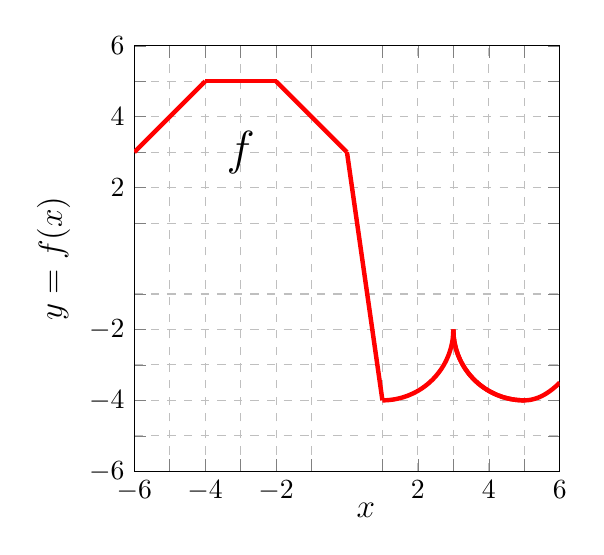
\begin{tikzpicture}[scale=1]
          \begin{axis}[
        %    axis y line = left,
        %    axis x line = bottom,
            xlabel = {\large$x$},
                            xlabel style={anchor=west},
            ylabel = {\large$y=f(x)$},
                            ylabel style={anchor=south},
            xtick       = {-6,-5, -4, -3,-2,-1,1,2,3, 4, 5, 6},
            xticklabels = {$-6$, , $-4$, ,$-2$,,,$2$,, $4$, , $6$},
            ytick       = {-6,-5, -4, -3,-2,-1,1,2,3, 4, 5, 6},
            yticklabels = {$-6$, , $-4$, ,$-2$,,,$2$,, $4$, , $6$},
            samples     = 160,
            domain      = 0:3,
            restrict y to domain=-10:100,
            xmin = -6, xmax = 6,
            ymin = -6, ymax = 6,
            width=2.75in,height=2.75in,
            grid=both, grid style=dashed
          ]
          %
          \addplot[domain=-6:-4, red, ultra thick, mark=none] {x + 9};
          %
          \addplot[domain=-4:-2, red, ultra thick, mark=none] {5};
          %
          \addplot[domain=-2:0, red, ultra thick, mark=none] {-x + 3};
          %
          \addplot[domain=0:1, red, ultra thick, mark=none] {-7*x+3};
          \addplot[domain=1:3, red, ultra thick, mark=none] {-2 - (4 - (x-1)^2)^(0.5)};
          \addplot[domain=3:5, red, ultra thick, mark=none] {-2 - (4 - (x-5)^2)^(0.5)};
          \addplot[domain=3:5, red, ultra thick, mark=none] {-2 - (4 - (x-5)^2)^(0.5)};
          \addplot[domain=5:6, red, ultra thick, mark=none] {-4 + 0.5*(x-5)^2};
          %
          \filldraw[black] (-3,3) circle (0pt) node[] {\LARGE $f$};
        \end{axis}
    \end{tikzpicture}  
    }{\centering
      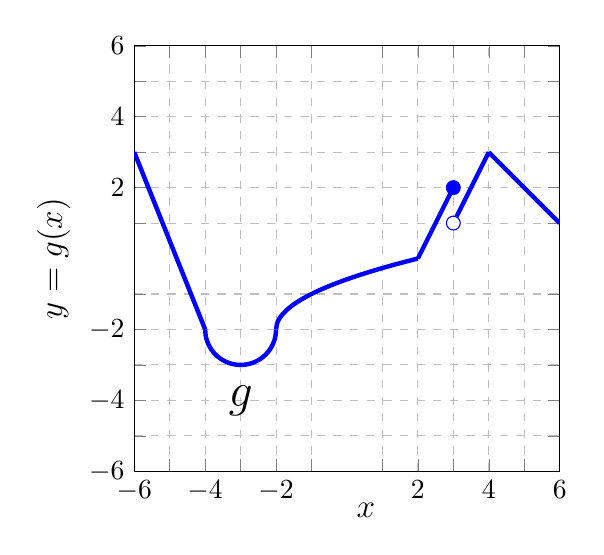
\begin{tikzpicture}[scale=1]
          \begin{axis}[
        %    axis y line = left,
        %    axis x line = bottom,
            xlabel = {\large$x$},
                            xlabel style={anchor=west},
            ylabel = {\large$y=g(x)$},
                            ylabel style={anchor=south},
            xtick       = {-6,-5, -4, -3,-2,-1,1,2,3, 4, 5, 6},
            xticklabels = {$-6$, , $-4$, ,$-2$,,,$2$,, $4$, , $6$},
            ytick       = {-6,-5, -4, -3,-2,-1,1,2,3, 4, 5, 6},
            yticklabels = {$-6$, , $-4$, ,$-2$,,,$2$,, $4$, , $6$},
            samples     = 160,
            domain      = 0:3,
            restrict y to domain=-10:100,
            xmin = -6, xmax = 6,
            ymin = -6, ymax = 6,
            width=2.75in,height=2.75in,
            grid=both, grid style=dashed
          ]
          %
%          \addplot[domain=-6:-4, red, ultra thick, mark=none] {x + 9};
%          %
%          \addplot[domain=-4:-3, red, ultra thick, mark=none] {5};
%          %
%          \addplot[domain=-3:0, red, ultra thick, mark=none] {-2/3 * x + 3};
%          %
%          \addplot[domain=0:1, red, ultra thick, mark=none] {-7*x+3};
%          \addplot[domain=1:3, red, ultra thick, mark=none] {-2 - (4 - (x-1)^2)^(0.5)};
%          \addplot[domain=3:5, red, ultra thick, mark=none] {-2 - (4 - (x-5)^2)^(0.5)};
%          \addplot[domain=3:5, red, ultra thick, mark=none] {-2 - (4 - (x-5)^2)^(0.5)};
%          \addplot[domain=5:6, red, ultra thick, mark=none] {-4 + 0.5*(x-5)^2};
%          %
%          \filldraw[black] (-3,3) circle (0pt) node[] {\LARGE $f$};
          %
          %\draw[->,thick] (-0.9,1.9) -- (-0.35,1.6);
          %
          \addplot[domain=-6:-4, blue, ultra thick, mark=none] {-5/2 *x -12};
          %
          \addplot[domain=-4:-2, blue, ultra thick, mark=none] {-2 - (1 - (x+3)^2)^(1/2)};
          \addplot[domain=-2:2, blue, ultra thick, mark=none] {(x+2)^(1/2) - 2};
          %
          \addplot[domain=2:3, blue, ultra thick, mark=none] {2*x-4};
          \addplot[domain=3:4, blue, ultra thick, mark=none] {2*x-5};
          \filldraw[white] (3,1) circle (2.5pt);
          \draw[blue] (3,1) circle (2.5pt);
          \filldraw[blue] (3,2) circle (2.5pt);
          \addplot[domain=4:6, blue, ultra thick, mark=none] {-x+7};
          %
          \filldraw[black] (-3,-4) circle (0pt) node[] {\LARGE $g$};
          %
          %\draw[->,thick] (0.3,-1.5) -- (-0.2,-1.3);
          %
        \end{axis}
    \end{tikzpicture}    
}
\item  Let $k(x)=f(g(x))$, where $f$ and $g$ are functions whose graphs are shown below. \\ What are the following values?
\tasksA{2}{
\task  $k'(-3)$
\task $k'(5)$
}

\mpageT{.5}{.5}{
\centering
    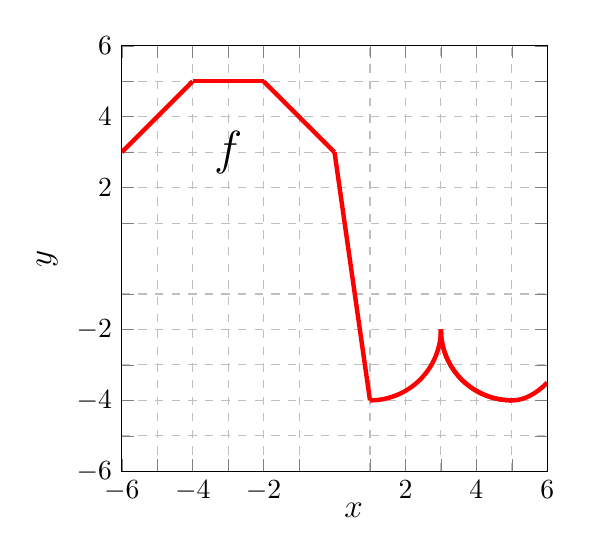
\begin{tikzpicture}[scale=1]
          \begin{axis}[
        %    axis y line = left,
        %    axis x line = bottom,
            xlabel = {\large$x$},
                            xlabel style={anchor=west},
            ylabel = {\large$y$},
                            ylabel style={anchor=south},
            xtick       = {-6,-5, -4, -3,-2,-1,1,2,3, 4, 5, 6},
            xticklabels = {$-6$, , $-4$, ,$-2$,,,$2$,, $4$, , $6$},
            ytick       = {-6,-5, -4, -3,-2,-1,1,2,3, 4, 5, 6},
            yticklabels = {$-6$, , $-4$, ,$-2$,,,$2$,, $4$, , $6$},
            samples     = 160,
            domain      = 0:3,
            restrict y to domain=-10:100,
            xmin = -6, xmax = 6,
            ymin = -6, ymax = 6,
            width=2.75in,height=2.75in,
            grid=both, grid style=dashed
          ]
          %
          \addplot[domain=-6:-4, red, ultra thick, mark=none] {x + 9};
          %
          \addplot[domain=-4:-2, red, ultra thick, mark=none] {5};
          %
          \addplot[domain=-2:0, red, ultra thick, mark=none] {-x + 3};
          %
          \addplot[domain=0:1, red, ultra thick, mark=none] {-7*x+3};
          \addplot[domain=1:3, red, ultra thick, mark=none] {-2 - (4 - (x-1)^2)^(0.5)};
          \addplot[domain=3:5, red, ultra thick, mark=none] {-2 - (4 - (x-5)^2)^(0.5)};
          \addplot[domain=3:5, red, ultra thick, mark=none] {-2 - (4 - (x-5)^2)^(0.5)};
          \addplot[domain=5:6, red, ultra thick, mark=none] {-4 + 0.5*(x-5)^2};
          %
          \filldraw[black] (-3,3) circle (0pt) node[] {\LARGE $f$}; 
        \end{axis}
    \end{tikzpicture}   
    }{ \centering
     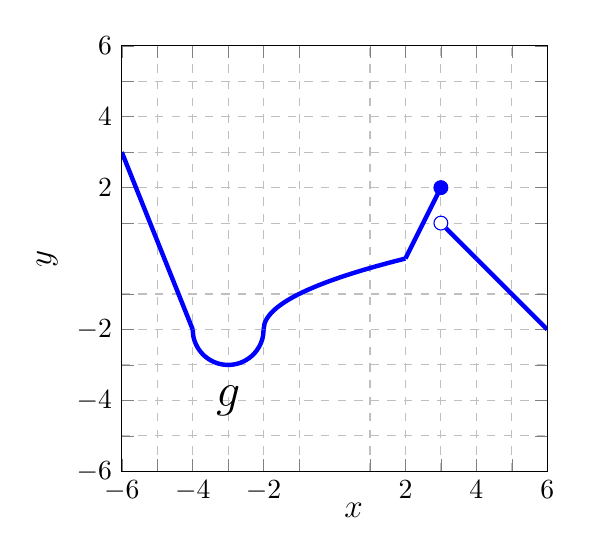
\begin{tikzpicture}[scale=1]
          \begin{axis}[
        %    axis y line = left,
        %    axis x line = bottom,
            xlabel = {\large$x$},
                            xlabel style={anchor=west},
            ylabel = {\large$y$},
                            ylabel style={anchor=south},
            xtick       = {-6,-5, -4, -3,-2,-1,1,2,3, 4, 5, 6},
            xticklabels = {$-6$, , $-4$, ,$-2$,,,$2$,, $4$, , $6$},
            ytick       = {-6,-5, -4, -3,-2,-1,1,2,3, 4, 5, 6},
            yticklabels = {$-6$, , $-4$, ,$-2$,,,$2$,, $4$, , $6$},
            samples     = 160,
            domain      = 0:3,
            restrict y to domain=-10:100,
            xmin = -6, xmax = 6,
            ymin = -6, ymax = 6,
            width=2.75in,height=2.75in,
            grid=both, grid style=dashed
          ]
          %
%          \addplot[domain=-6:-4, red, ultra thick, mark=none] {x + 9};
%          %
%          \addplot[domain=-4:-3, red, ultra thick, mark=none] {5};
%          %
%          \addplot[domain=-3:0, red, ultra thick, mark=none] {-2/3 * x + 3};
%          %
%          \addplot[domain=0:1, red, ultra thick, mark=none] {-7*x+3};
%          \addplot[domain=1:3, red, ultra thick, mark=none] {-2 - (4 - (x-1)^2)^(0.5)};
%          \addplot[domain=3:5, red, ultra thick, mark=none] {-2 - (4 - (x-5)^2)^(0.5)};
%          \addplot[domain=3:5, red, ultra thick, mark=none] {-2 - (4 - (x-5)^2)^(0.5)};
%          \addplot[domain=5:6, red, ultra thick, mark=none] {-4 + 0.5*(x-5)^2};
%          %
%          \filldraw[black] (-3,3) circle (0pt) node[] {\LARGE $f$};
          %
          %\draw[->,thick] (-0.9,1.9) -- (-0.35,1.6);
          %
          \addplot[domain=-6:-4, blue, ultra thick, mark=none] {-5/2 *x -12};
          %
          \addplot[domain=-4:-2, blue, ultra thick, mark=none] {-2 - (1 - (x+3)^2)^(1/2)};
          \addplot[domain=-2:2, blue, ultra thick, mark=none] {(x+2)^(1/2) - 2};
          %
          \addplot[domain=2:3, blue, ultra thick, mark=none] {2*x-4};
          \addplot[domain=3:4, blue, ultra thick, mark=none] {-x+4};
          \filldraw[white] (3,1) circle (2.5pt);
          \draw[blue] (3,1) circle (2.5pt);
          \filldraw[blue] (3,2) circle (2.5pt);
          \addplot[domain=4:6, blue, ultra thick, mark=none] {-x+4};
          %
          \filldraw[black] (-3,-4) circle (0pt) node[] {\LARGE $g$};
          %
          %\draw[->,thick] (0.3,-1.5) -- (-0.2,-1.3);
          %
        \end{axis}
    \end{tikzpicture}
}
\end{enumerate}
    \newpage
    \section{Conceptual Derivatives}
    
    
Let $f(x)$ and $g(x)$ be functions with the following values:$$
\begin{array}{|c|c|c|c|c|}
\hline
x & f(x) & f'(x) & g(x) & g'(x) \\
\hline
0 & 0 & -1 & 2 & 1/2 \\
1 & 1 & -2 & 0 & 0\\
\hline
\end{array}
$$
Compute the following derivatives. Try to identify the outermost functions, then break them down to find each derivative separately.
\tasksE{2}{
    \task $\ds \frac{d}{dx} \left[ \frac{ (f(1-x))^2 }{ x^3 + 1 } \right]_{x=1}$
    \task $\ds \frac{d}{dx} \left[ f(x^2 - 1) \cdot g(2x - 1) \right]_{x=1}$
    \task $\ds \frac{d}{dx} \left[ \frac{f(x^2-2x+1)}{\sqrt{g(x) + 5}} \right]_{x=1}$
}
    

    
%    \newpage
%\begin{enumerate}
%\item[Board 1.] \, 
%  
%\newpage 
%
%\item[Board 2.] \,  
%    \begin{enumerate}
%    \item $\dfrac{d}{dt}[ t^5 + 2t + 5]$
%    \item $\ds \dfrac{d}{dt}\left[\frac{5\sqrt{t}}{t^5+2t+5}\right]$
%    \item $\dfrac{d}{dt}\left[(t^3 + 2t^2)(t^3 - 2t^2)\right]$
%    \item $\ds \dfrac{d}{dt}\left[ g(e^{3t})\right]_{t=0}$  where $g(0)=-3$, $g(1)=5$, $g^{\prime}(0)= -7$, $g^{\prime}(1)= 9$ 
%    \end{enumerate}
%\newpage
%
%\item[Board 3.] \,  
%    \begin{enumerate}
%    \item $\ds \dfrac{d}{dx}\left[e^{5x^2+7}\right]$
%    \item $\ds \dfrac{d}{dx}\left[\frac{e^x}{3x^2}\right]$
%    \item $\dfrac{d}{dx}\left[(x + 1)(x - 1)(x+1)\right]$
%    \item $\ds \frac{d}{dx} \left[ f(x^3+2) \right]_{x=2}$ where $f(2)=-3$, $f(10)=5$ $f^{\prime}(2)=-7$ and $f^{\prime}(10)=9$
%    \end{enumerate}
%    \newpage 
%    
%\item[Board 4.] \,  
%    \begin{enumerate}
%
%\item $\ds \frac{d}{dx}\left[(x^4-\sqrt{x}+2)^6 \right]$
%    \item $\ds \dfrac{d}{dx}\left[\frac{x^3+2x+9}{\sqrt{x}}\right]$
%    \item $\dfrac{d}{dx}\left[e^x \sqrt{x}\cdot x\right]$
%        \item $\ds \dfrac{d}{dx}\left[x^2f(x) \right]_{x=2}$ where $f(2)=3$, $f^{\prime}(2)=7$
%    \end{enumerate}
%    \newpage
%    
%\item[Board 5.] \,  
%    \begin{enumerate}
%            \item $\dfrac{d}{dt}[2\sqrt{t}-t]$
%    \item $\dfrac{d}{dx}[(x^2 + 9x)(3x^2+10)]$
%    \item $\ds \dfrac{d}{dx}\left[\frac{1}{3\sqrt{6x-5}}\right]$
%        \item $\ds \dfrac{d}{dx}\left[\frac{f(x) + e^x}{\sqrt{x}}\right]_{x=4}$ where $f(4)=-1$ and $f^{\prime}(4)=-5$
%    \end{enumerate}
%\newpage
%
%\item[Board 6.] \,  
%    \begin{enumerate}
%    \item $\ds \dfrac{d}{dt}[5\sqrt{t} + 9]$
%    \item $\ds \dfrac{d}{dt}\left[\frac{\sqrt{t} + t^2 + t}{t^9}\right]$
%    \item $\dfrac{d}{dt}\left[e^x + e^x + e^9\right]$
%        \item $\ds \dfrac{d}{dt} \left[f(t) + \frac{f(t)}{t^3}\right]_{t=3}$ where $f(3)=2$ and $f^{\prime}(3)=4$
%    \end{enumerate}
%\newpage
%
%\item[Board 7.] \,
%    \begin{enumerate}
%    \item $\dfrac{d}{dx}[\sqrt{x} + 3\sqrt{x} + \sqrt[3]{x}]$
%    \item $\ds \frac{d}{dx}\left[\frac{\sqrt[3]{x}}{x^9+x^8+5}\right]$
%    \item $\dfrac{d}{dt}\left[\pi + e^{100} + \pi^{e^\pi}\right]$
%        \item $\ds \dfrac{d}{dt}\left[\frac{g(t)}{f(t)} + f(t)\right]_{t=-1}$ where $f(-1)=2$, $f^{\prime}(-1)=3$, $g(-1)=4$ and $g^{\prime}(-1)=5$
%    \end{enumerate}
%    
%   \newpage
%\item[Board 8.] \,
%    \begin{enumerate}
%    \item $\ds \dfrac{d}{dx}\left[\frac{x^2}{f(x)}\right]\bigg\rvert_{x = 4}$ where $f(4) = 3$ and $f'(4) = -1$
%    \item $\dfrac{d}{dt}[(2f(x)+9)(g(x) - 5)]\bigg\rvert_{x = 3}$ where $f(3) = 7, f'(3) = 5, g(3) =4, g'(3) = 6$
%    \item $\ds \frac{d}{dx}\left[f(x^2)\right]\bigg \rvert_{x = 3}$ where $f(9) = 6, f'(9) = 7$
%    \end{enumerate}
%
%\newpage
%\item[Board 9.] \,
%    The following derivative will need to be computed in a few steps. What should be done first? Discuss with your group. What do you suspect will be the next rules you need?
%    $$\frac{d}{dt} \frac{(t+1)(t-1)}{\sqrt{t} + \sqrt[3]{t}}.$$
%    Compute the derivative and check against your first answers.
%\end{enumerate}

}


\end{document}